\chapter{Risks \& Safety}\label{5_chap:safety}
\section{Risks}
The maximum sound pressure level that is allowed by \acrshort{suva} is $140 \,$dB and the averaging level 8h/day has to be below $110 \,$dB. The averaging level $L_m$ is given as
\begin{equation}\label{5_Safety_eq:AveragingLevel}
    L_m = 10 \log_{10} \left (  \frac{1}{8} \int_0^T 10^{0.1 L_p(t)}dt\right ).
\end{equation}
This can be solved for the sound pressure level $L_p(t) = L_p$ if it is assumed to be constant over a certain time $\tau$
\begin{equation}\label{5_Safety_eq:AveragingLevel_SPL}
    L_p = L_m - 10\log_{10}\left ( \frac{\tau}{8} \right ).
\end{equation}
To calculate the sound pressure level at any given point, the directivity of the used transducers has to be calculated. As explained in Section \ref{3_sec:directivity}, the sound directivity can be calculated as
\begin{equation}\label{5_Safety_eq:Directivity}
    Q_D = \frac{2 p(0)^2}{\int_{0}^{\pi}p^2(\theta)\sin{\theta}d\theta}. 
\end{equation}
The sound pressure ratio emitted by the transducers according to its datasheet is displayed in Figure \ref{5_fig:directivity_transducer}.
\begin{figure}[h!]
    \centering
    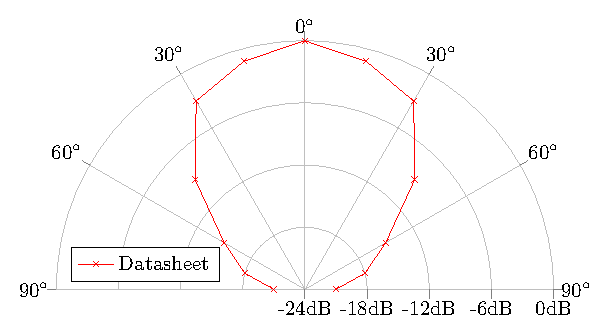
\includegraphics[width=0.72\textwidth]{images/5_Safety_Risks/Polar_PlotDirectivity.pdf}
    \caption{Directivity of a Transducer}
    \label{5_fig:directivity_transducer}
\end{figure}
\newpage

With this information, the directivity index results to be $Q_D = 22$. This then can be used to calculate the maximum allowed sound power level in relation to the distance of the listener 
\begin{equation}
         L_{wmax} 
     = 
     \underbrace{L_{pmax}}_{140dB} - 10\left ( \underbrace{\log_{10}(Q_D)}_{1.35B} - \log_{10}(r^2) - \underbrace{\log_{10}(4\pi)}_{\approx 1.1B}  \right ) = 137.5 + 20\log_{10}(r).
     \label{5_eq:safety_max}
\end{equation}

The maximum sound power allowed in relation to the distance is plotted in Figure \ref{5_Safety_fig:Max_power_allowed}.
\begin{figure}[h!]
    \begin{minipage}{0.49\textwidth}
        \centering
        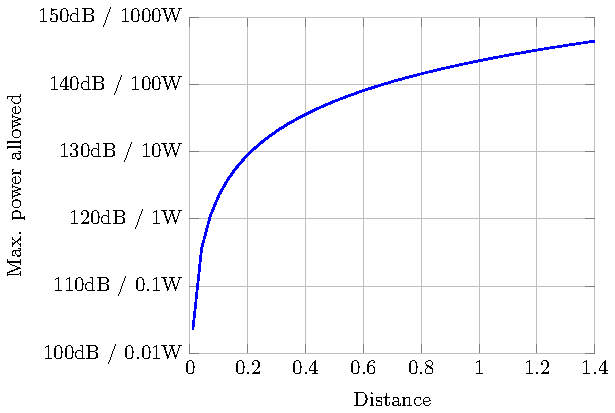
\includegraphics[width=\textwidth]{images/5_Safety_Risks/Max_Power_Allowed.pdf}
        \caption{Maximum allowed Sound Power}
        \label{5_Safety_fig:Max_power_allowed}
        \end{minipage}
    \begin{minipage}{0.49\textwidth}
        \centering
        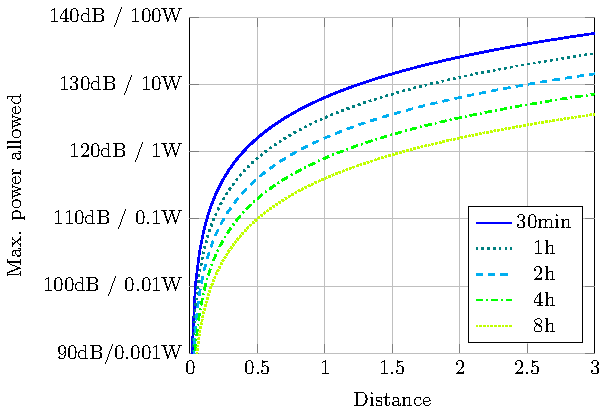
\includegraphics[width=\textwidth]{images/5_Safety_Risks/Max_Power_Allowed_Time.pdf}
        \caption{Maximum Power allowed (daily)}
        \label{5_Safety_fig:Max_power_allowed:daily}
    \end{minipage}
\end{figure}
In Figure \ref{5_Safety_fig:Max_power_allowed:daily} the maximum sound power allowed over different periods of time is shown. This was calculated by using Equation \ref{5_Safety_eq:AveragingLevel_SPL} and Equation \ref{5_eq:safety_max} where $L_m = 110\,dB$ as stipulated by \acrshort{suva}.  

\newpage
\section{Safety}
Through measuring the voltage over a resistor $R$ right in front of each line of transducer arrays, the total current going into the transducers could be measured. Additionally the voltage over the transducers was measured. From these measurements the total possible sound power which the whole transducer array could produce can be calculated
\begin{equation}
    L_{P,max} = M \cdot \frac{U_R}{R} U_{T}\eta_{T}.
\end{equation}
Where M is the number of channels, $U_R$ is the voltage over the resistor, $U_T$ is the voltage over the transducer and $\eta_{T}$ is the efficiency of the transducer. To guarantee maximal safety, the efficiency $\eta_{T}$ is assumed to be one, which is highly overestimated.
In this particular case the number of channels is $M = 19$. For the transducers the voltages measured were $U_R = 1.78 \, V$ and $U_T = 9.5 \, V $ and the resistor is $R = 22 \, \Omega$. This can be used to calculate the maximum sound power
\begin{equation}
     L_{P,max} = 19 \cdot \frac{1.78 V}{22 \Omega} 9.5 V = 14.36 \, \text{W}
\end{equation}
So, to guarantee that a person could listen to the Audio-Beamformer on full volume for half an hour daily without any harm, the minimum distance was calculated using Equation \ref{5_Safety_eq:AveragingLevel_SPL} and Equation \ref{5_eq:safety_max} to be 2.5 meters. The minimum distance was set to 2.5 meters. This distance is measured by a \acrfull{tof} sensor, the implementation of this is explained in Section \ref{4_Sensors_Near-field}.     
\newpage